\chapter{Write Away 1}

\begin{figure}[H]
    \centering
    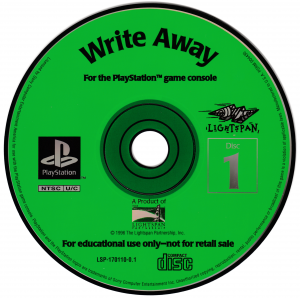
\includegraphics[width=\textwidth/2]{./Games/WriteAway/Images/WriteAway1CD.png}
    \caption{Write Away 1 CD}
\end{figure}

The first of the ten Write Away games published and released by The Lightspan Partnership for the PlayStation 1.

Write Away 1 features ten video programs, including an introduction video, eight story videos, and a conclusion video:

\begin{itemize}
    \item Write Away Episode One Introduction
    \item The Magic Umbrella by Deeana Downes
    \item In My Desk by Jonathan Garcia
    \item Baby Nathan by Mrs. Brozda's Second Grade Class
    \item Wonder Parrot by Derek Lawson
    \item The Butterfly Basket by Anne McCorkhill
    \item Team Work by Zachary Frank
    \item The Mixed Up Googles by Anna Bell and Sarah Berryman
    \item The Boy Who Went Into Space by Nicolas Allen
    \item Write Away Conclusion
\end{itemize}

\clearpage
\newpage

\section{Transcriptions}

\subsection{The Magic Umbrella by Deeana Downes}

SABRINA: Come on! Come out genie!

JOE: Sabrina what's wrong?

SABRINA: I've been rubbing and rubbing this lamp and it just doesn't work.
I guess there's no such thing as magic lamps.

JOE: Well this lamp might not be magic but as an author, you can create magic anytime you want, just by using your imagination.
Just look at what magic our second grade author Deanna Downs from Town Point School created in her story called 'The Magic Umbrella'.
Once upon a time there was a little girl who wanted a magic umbrella.

GIRL: If only I had a magic umbrella, then I could fly anywhere in the whole wide world!
Mom and dad, may I please have a magic umbrella?

MOM AND DAD: A magic umbrella?

GIRL: Yeah, see if I had a magic umbrella, then I could fly anywhere in the whole wide world.

DAD: All right, let's go to the store and get one!

JOE (VOICE OVER): So the little girl's parents took her to the store.
At the store, she saw all sorts of umbrellas and she liked them all very much.

GIRL: Mom! Mom!
May I have one of these?

MOM: Oh, these are much too expensive.
If you want one, you'll have to earn the money yourself.

GIRL: I will earn the money!

JOE (VOICE OVER): So every day after school, the little girl would help people and earn money.

WOMAN 2: Oh thank you so much for washing my dog and mowing my lawn!
It looks fabulous, here's your money.

GIRL: Nine, ten... yes!
Now I have enough money to buy my new magic umbrella!

JOE (VOICE OVER): So the little girl went back to the store to buy her magic umbrella.

STORE OWNER: Hi, which one would you like?

GIRL: Well, I want a magical umbrella!

STORE OWNER: Well, they're all magical.

GIRL: Oh, I'll take that one.

STORE OWNER: Ten dollars.

JOE (VOICE OVER): She took it home and every night when the moon was high, she would fly around the world.

GIRL: Look mom and dad.
I'm flying!

MOM AND DAD: Nah.

\subsection{In My Desk by Jonathan Garcia}

ELISE:
Have you ever sat in class when the teacher says: 'all right class, let's clean out our desks!'
Does it make you shudder, cause you don't know what's in there.
Well, fifth grader Jonathan Garcia from Handy Elementary lets us share in his experience in the form of a poem entitled In My Desk.

BOY:
In my desk is a creepy old thing,

In my desk my cousin lost her ring.

In my desk I'm afraid to take a look,

I'm even scared to take out a book.

In my desk, I think something is in there,

Because there's lots and lots of hair.

In my desk there's too much stuff,

to get out a pencil is really really rough.

TEACHER:
All right class, it's time to take out your pencils!

BOY:
In my desk... The end.

\subsection{Baby Nathan by Mrs. Brozda's Second Grade Class}

DEBORAH:
Joe, what are you doing?
You're making a mess!

JOE:
Well, I've been trying to write a story but I just don't know what to write about.

DEBORAH:
Well, one way to get started with a story is to write about something or someone you already know.

JOE:
Something or someone I already know?
Hey, I know, I'll write about me!
Once upon a time, there was a handsome young boy named Joe.
Yeah, sounds good!

DEBORAH:
You see, sometimes it is easier when you write about someone you know.
And that's exactly what a group of second graders did.
They're from Mrs. Brozda's class at King's Elementary, and they wrote about a very special small person that they all know, named Baby Nathan.

GIRL 1:
Hi!
In our class, we have a very special person, but he's not a student.
He's a baby inside Miss Alcorn, our teacher's name.
She has been pregnant the whole school year.

TEACHER:
Or so it seems.

GIRL 1:
At first, it was a secret, but then she told the whole class,.

TEACHER:
Class, I have some wonderful news.
I'm going to have a baby, and it's going to be a baby boy, and I'm going to name him Nathan.

BABY NATHAN:
Yeah, and I can't wait to see the world.
Hey, more pickles down here!
I'm hungry!

GIRL 1:
We were so excited, we all shouted, 'yay!'
Then she showed us a picture of Nathan, a sonogram.

TEACHER:
You see, students, you can see his bones and his head and his arms and his legs.
It's a miracle!

GIRL 1:
Well, every day Miss Alcorn's stomach got bigger and bigger and bigger, and we would talk to Nathan inside.
Hi Nathan, how you doing?

BOY 1:
Hey guy, get your own swimming pool, huh?

GIRL 2:
Are you having fun?
Are you stuck in your thumb?
Are you awake?
Are you asleep?

GIRL 1:
Can you hear us in there?
We can't wait to see you for real!

BABY NATHAN:
Yeah, I can hear you, I can hear you.
Hey, more pizza down here!

TEACHER:
Oh, I think it's time to go to Pizza City!

CHILDREN:
Hello Baby Nathan, we love you so much!

BABY NATHAN:
Oh shucks!

GIRL 1:
Then one day, Miss Alcorn didn't come to school.
She had gone to the hospital to have her baby.
We all went to see him, and boy was he cute!
Cutie cutie cutie!
It was a miracle!
And that's all about Baby Nathan.

\subsection{Wonder Parrot by Derek Lawson}

SABRINA:
Elise, come over here and sit with me!

ELISE:
What?

SABRINA:
I can't wait to see this next story.

ELISE:
Why?
What's so special about this one?

SABRINA:
Well, you know how I love animal stories.

ELISE:
Yeah?

SABRINA:
This one was written by second grader Derek Lawson of Midland School.
As a writer, Derek took a normal pet and gave him some special abilities in his story 'Wonder Parrot'.

LUIGI:
Hello boys and girls, let me introduce myself to you.
Rawk!
I'm Luigi, I'm a bright colored bird, and I live on 66th Street.
I'm one smart bird.
I can talk and I could even use a telephone, which came in really handy one day.
Let me tell you how it all began.
It was such a nice day, rawk, when my owner Nick was playing with this ball.

MOM:
Nick, I'm going to the store, I'll be back in a few minutes.
Now stay away from the pool.

NICK:
Okay mom?

LUIGI:
Okay mom, rawk!

NICK:
Uh oh, I better get my ball out of the pool.

LUIGI:
Stay away from the pool, Nick, Rawk!
Well, Nick was getting closer and closer to the pool.
Watch out Nick, you're too close, rawk!

NICK:
I can reach it!
I can reach it!
Aah!

LUIGI:
Uh oh, Nick was in trouble.
I had to do something, so I jumped off my perch and I flew to the telephone.
I knocked out the receiver and I dialed 9-1-1.

EMERGENCY OPERATOR:
Hello, emergency operator?
How may I help you?

LUIGI:
Rawk, my name is Luigi!
My name is Luigi! Rawk!

EMERGENCY OPERATOR:
Well Luigi, you know it's against the law to call 911 without an emergency.

LUIGI:
Rawk!
Stupid operator!
Stupid operator!
Rawk!

EMERGENCY OPERATOR:
Well I never!
I'm going to send a police officer over there right now to find out who you are!

LUIGI:
Rawk! Right away, stupid!
Right away, stupid!
Rawk!

NICK:
Help! Help!

LUIGI:
Nick, I almost forgot.

NICK:
Help! Help!

LUIGI:
Suddenly the police woman arrived. Rawk!
'Uh oh, big trouble!
Big trouble!

POLICE WOMAN:
You are in big trouble!

LUIGI:
But then I had a brilliant idea.
I pointed my wing out the window. Rawk!

NICK:
Help!

LUIGI:
She saw Nick.
Then she ran and pulled him out of the pool.

POLICE WOMAN:
Now you were lucky to have such a smart parrot.
Now remember, never go near the pool without a parent!

LUIGI:
Rawk!

NICK:
Thanks Luigi, you saved the day!
I'm gonna buy you a brand new golden cage.

LUIGI:
Of course, cause I am Luigi the Wonder Parrot!

\subsection{The Butterfly Basket by Anne McCorkhill}

PAUL:
Hi, may look like I'm just eating an apple, but I can share this apple with you in words that will help you see how shiny red it is, and taste how deliciously sweet it is.
These words are known as adjectives, and a wonderful example of this can be seen from sixth grader Anne McCorkhill from Mountain View School, and her story entitled 'The Butterfly Ballet'.

WOMAN 1:
As I floated in the field of beautiful wild flowers, I could feel the silky green grass between my fingers.
I could hear the birds, they were singing in the sky and as I looked up into the sky, the clouds looked like an ocean and the scent of the wildflowers smell better than the best perfume in the world.
Oh [there is] a butterfly, I go to chase it.
I can taste the wind on my mouth as I ran.
And then suddenly, I felt myself change into a butterfly.
Oh, I felt as if I had all the time in the world.

Then I caught myself up in the clouds and the clouds felt like big soft fluffy pillows.
I decided to go back down into the wild flowers, and there I tasted the sweet nectar of the wild flowers.
But then, suddenly, like a snap, I started returning to my body.
I felt like, like I didn't belong there.
I tried to fly up into the sky, but my feet were caught to the ground, just like the nectar was caught to the tip of my tongue.

And then I was no longer sad or hurt because I knew that I could go back to that time any time I wanted to, just by shutting my eyes, and then I'd be back in the world of happiness.
The world of the butterfly - the butterfly ballet.
The end.

\subsection{Team Work by Zachary Frank}

THEME TUNE:
Pick up a paper and pen, write away.

ELISE:
You know a lot of stories are written just to entertain us.
But I really love stories that teach us lessons, lessons about how to be better people.
And our next story does just that.
It's written by fifth grader Zachary Frank of Crescent Intermediate, and it's called 'Team Work'.

ELISE (VOICE OVER):
Jimmy and Sue were brother and sister.
They were the fastest runners in the school.
In fact, no one could beat them at running relays.
Sue would start, and Jimmy would always run anchor.

JIMMY:
We can't be beat.

SUE:
We're the best!

ELISE (VOICE OVER):
However, one day, a new boy moved into the school named Johnny.

JOHNNY:
Can I race with you too?

JIMMY:
No!

JOHNNY:
Why not?

SUE:
Because we're the best, you know.
    [I mean] there's no one faster.

JIMMY:
Wait, if you could race me and win, then you can beat the relays with us.
But I don't think you can do it, 'cause no one else has.

ELISE (VOICE OVER):
Well, Johnny took the challenge.

SUE:
On your marks, get set, go!

ELISE (VOICE OVER):
He smoked Jimmy in the first hundred-meter heat.

JIMMY:
Hey, you started too soon!

ELISE (VOICE OVER):
Jimmy complained of Johnny jumping the gun.

SUE:
On your marks, get set, go.

ELISE (VOICE OVER):
So they ran it over and got the same results.
There was no doubt about it, Johnny was a lot faster than Jimmy.

SUE:
You know, Johnny, you're pretty fast.
I have an idea, the international relay race is coming up.
Let's join the three-person team relay.

JIMMY:
Well, that's a good idea, Sue, if you consider riding with us, Johnny.

JOHNNY:
Wow, sure!

ELISE (VOICE OVER):
So that's exactly what happened.
Sue continued to be the lead, her brother Jimmy took the second seat, and Johnny, the new boy in school, ran anchor.
They took home first place, and they continued to win races.
However, they are all well aware that another new child could come to school any day and challenge them for the fastest.
They all learned an important lesson.

SUE:
You may be good.

JOHNNY:
Even the best.

JIMMY:
But there's always someone better.

TOGETHER:
Team work!

\subsection{The Mixed Up Googles by Anna Bell and Sarah Berry}

DEBORAH:
You know it's a lot of fun when you write a story by yourself, but it can even be more fun when you write with someone else, and that's called a collaboration.
Now a collaboration is when two writers or more get together, put their ideas down on paper, and form a story.
And that's exactly what our next two authors did - kindergartner Anna Bell and fourth-grader Sarah Berryman.
They're from Alps Road School in Athens, Georgia, and they wrote a wonderful story entitled 'The Mixed-Up Googles'.

DEBORAH (VOICE OVER):
One day, in a kindergarten class, two little girls, Carly and Anna, were playing blocks when they heard a loud sound.

CARLY:
It sounded like something landed on the roof!

ANNA:
Well let's go check it out!

DEBORAH (VOICE OVER):
But before they could even get out the door, two strange-looking creatures walked in.

CARLY AND ANNA:
Aah!

LIMI:
Hey, don't be afraid, I'm Limi.

SCREAMY:
And I'm Screaming.

LIMI:
We're Google monsters.

SCREAMY:
And we want to become human.

CARLY:
Well, well we can teach you everything we know about being human.

LIMI AND SCREAMY:
Okay!

DEBORAH (VOICE OVER):
So Anna and Carly tried to teach them how to be human.
First, they showed them how to tie their shoes.

CARLY AND ANNA:
Aah!

LIMI AND SCREAMY:
Uh oh.

DEBORAH (VOICE OVER):
Next, they showed them how to drink milk.
And then they showed them how to build blocks.

LIMI AND SCREAMY:
Uh oh.

CARLY:
This just isn't working.
You're Googles, and we're humans.

ANNA:
I think you should just be yourselves.

LIMI:
But we want to be like humans.

SCREAMY:
We want to be like you.

LIMI AND SCREAMY:
We want to be like - waa aah

LIMI:
Hey, wait a minute, they're right, we're Googles.
We should just be ourselves after all.

SCREAMY:
After all, we're smart and very handsome.

CARLY:
I think we should all be happy with who we are.

LIMI:
Oh, it's time to go now.

SCREAMY
We'll never forget you.

LIMI:
Um, instead of being humans, it's better to be friends with humans.
Bye!

DEBORAH (VOICE OVER):
So the monsters left as quickly as they came, and Anna and Carly went back to what they like doing best - playing and just being themselves.

\subsection{The Boy Who Went Into Space by Nicolas Allen}

DEBORAH:
Sabrina, those were two of the funniest monsters I've ever seen.

SABRINA:
They sure were strange.
I think it's fun to see how two authors can write about aliens in completely different ways.
Third-grader Nicholas Allen from Lakeview Elementary wrote about another kind of alien in his story 'The Boy that Went into Space'.
Let's see what he did.

DEBORAH (VOICE OVER):
Once upon a time, there was a boy named Victor who loved to watch his father work.
That's because his father had a very important job.

VICTOR:
Wow, Dad, I've bet I'm the only boy whose father works on the space shuttle.

DAD:
I have a very important job, son.
Without me, those spaceships wouldn't fly.

VICTOR:
Is the toaster fixed yet, Dad?

DAD:
Not yet son.

DEBORAH (VOICE OVER):
One day, Victor went with his dad to watch him work on a spaceship.

VICTOR
Wow, Dad, this is neat, so many dials and buttons.

DAD:
That's right, son, but be very careful.
Whatever you do, don't touch that button marked 'blast off'.

VICTOR:
Okay?

DAD:
Oh, I'll be right back.
They're low on that orange drank.

VICTOR:
I'll just go out this window in and - oh no!

LAUNCH ANNOUNCER:
And liftoff. Liftoff.

VICTOR:
Help! Help! Help!

DEBORAH (VOICE OVER):
[It] was too late.
Victor was trapped inside the space shuttle, and it took off!
He flew and flew until he landed on a planet.

DAD:
Son, don't worry, you'll be all right, and I fixed the toaster.

VICTOR:
Wow, Dad, that's great.
Oh, I decided to explore the planet for life forms.
Don't worry, Dad.

DEBORAH (VOICE OVER):
Victor walked around the planet and got lost.
Suddenly, an alien appeared.

ALIEN:
Pidi pidi.

VICTOR:
What?
I don't understand you.
My name is Victor.
I'm from Earth.

ALIEN:
Pidi pidi pi.

VICTOR:
Aah!

DEBORAH (VOICE OVER):
The alien grabbed Victor and tied him up.
Then, she began to yell at Victor in Martian.

ALIEN:
Pidi pidi pi pidi pidi pi pidi pidi pi pidi pi.

VICTOR:
I don't understand you.
I'm Victor from Earth.
Victor.

DEBORAH (VOICE OVER):
The Martian got frustrated and walked away.

ALIEN:
Pidi pidi pi pidi pidi pi pidi pidi pi pidi pi.

VICTOR:
My chance to escape!

DEBORAH (VOICE OVER):
Victor began to run, but the Martian saw him and began to chase him everywhere.
Suddenly, the Martian pulled out a laser gun and was just about to zap Victor when...

DAD:
Wake up!
Victor!

VICTOR:
Don't shoot me!
Don't shoot me!
Don't shoot me!
Oh...

DAD:
Victor! You'll be late for school.

VICTOR:
Oh, dad I had the most horrible dream.
I was up in space, and like, 'shhh', and then the little Martian was like 'eh ha, eh ha', and it was going to shoot me, and then I woke up.

DAD:
There's no such thing as Martians.

VICTOR:
Oh, thank goodness it was only a nightmare.

ALIEN:
Eh dor!

VICTOR:
Aah!

\subsection{Write Away Conclusion}
DEBORAH:
We hope you enjoyed our show today.
Your stories are finished and all put away

JOE:
But we'll come again another day.

SABRINA:
The stories you've seen through music and mind -

ELISE:
- Can be written by you if you just take the time.

PAUL:
So get out a pen and paper, you'll see.

EVERYONE:
The adventures and magic that writing sets free.

DEBORAH:
We really had some great stories today.

JOE:
And we had a lot of fun acting them out.

DEBORAH:
But we're going to need a lot more for the months to come.

SABRINA:
You can write alone or with somebody else. Write about anything you want.

JOE:
So just take those words inside your head and put them down on a piece of paper, and send them in to us as soon as you can.

ELISE:
Who knows, you might even see your stories come to life. So...

EVERYONE:
Write away!

\section{Credits}